Now that the light potentials have been measured, we elaborate in this chapter how it was implemented in an real-world experiment on ultra-cold atoms, initially using Rb atoms.
In order to do this, a new setup was constructed.
The focus of the new machine was to have an optical setup as compact as possible.
The construction of the vacuum and atom source part can be found in \cref{sec:VacuumAtom}.
The laser system is explained in \cref{sec:LaserSystem}.
Images of the MOT are displayed in \cref{sec:MOTresult}.
We finish up with how overlap this MOT with our tweezer array (\cref{sec:Tweezers}) and how to image the tweezers (\cref{sec:TweezerImaging}).

\section{Vacuum and Atom Source}\label{sec:VacuumAtom}

The core of the experiment is the glass cell (30 mm outer and 4.0 mm wall thickness, optically contacted)\footnote{The glass cell was provided to us by our collaborators from the University of Amsterdam.}.
The glass cell can be seen in a CAD drawing and in real life in \cref{fig:VacuumSetup,fig:CoilsSetup}.
It is pumped down to the ultra-high vacuum regime, which is need to minimize collisions with the background gas and improve the lifetime of the atoms in the tweezers.
To pump the cell down, the glass cell is connected to a vacuum chamber (\cref{fig:VacuumSetup}, left).
We attach a turbomolecular pump to the chamber using a valve (not shown in the figure) and pump down to $\sim 10^{8}$ mbar.
This pressure was measured using a gauge attached on 
To reach a better vacuum, the system was baked for a duration of two weeks at 130${}^{\circ}$C by Rik van Herk \cite{Herk2022}.
Next, we activate the non-evaporative getter\footnote{NEXTorr Z 100 NEG - ion combination pump.} by heating it to 500${}^{\circ}$C while pumping away its outgassing using the turbo pump
Finally, after closing the turbo valve and turning on the ion pump we reached a pressure of $\sim 2\times 10^{-10}$ mbar.


As atom source, a triplet of Rubidium dispensers are used, powered by a power supply typically running at 5 ampères

The vacuum vessel and pump connections were performed by Rik van Herk and Deon Janse van Renseburg.
This is described in the thesis of Rik van Herk \cite{Herk2022}.


\begin{figure}
	\begin{subfigure}{.54\linewidth}
		\centering
		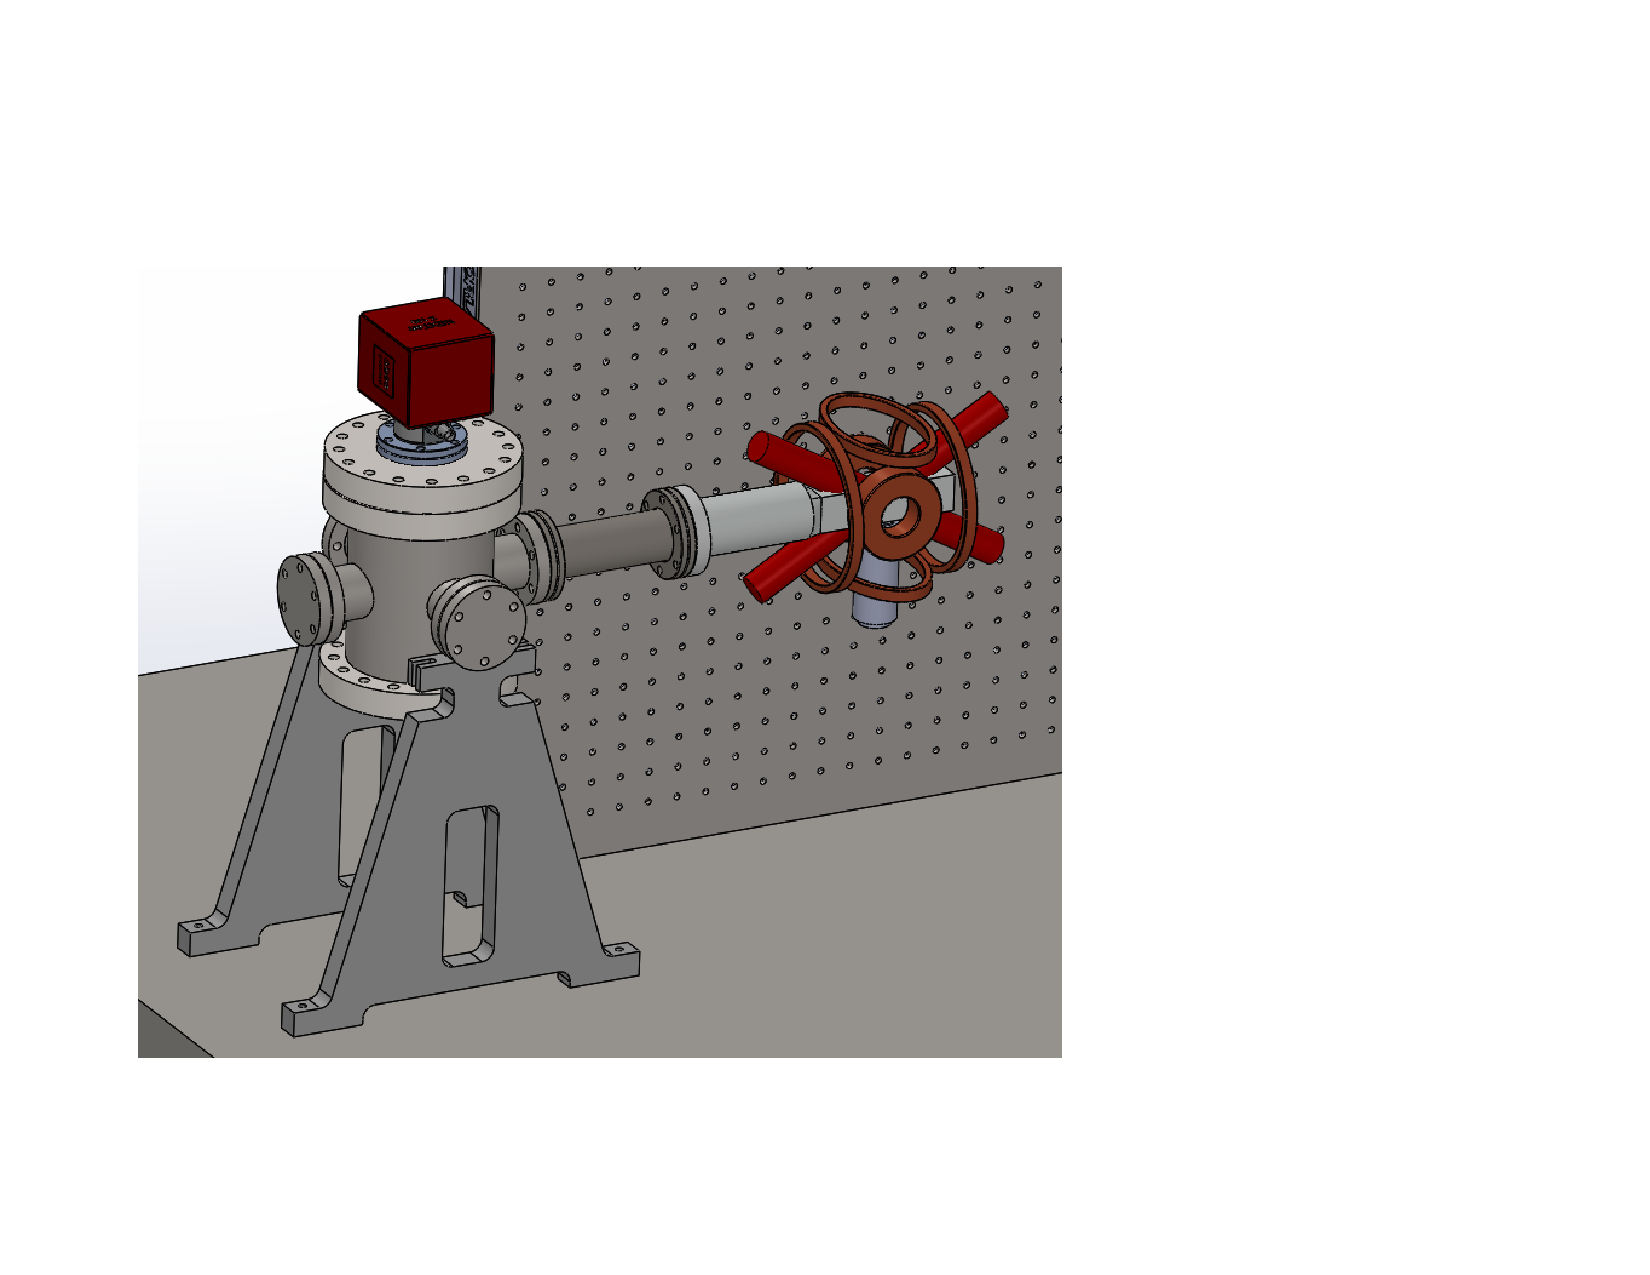
\includegraphics[height=6cm]{figures/Vacuum.pdf}
		\caption{}
		\label{fig:VacuumSetup}
	\end{subfigure}
	\hfill
	\begin{subfigure}{.44\linewidth}
		\centering
		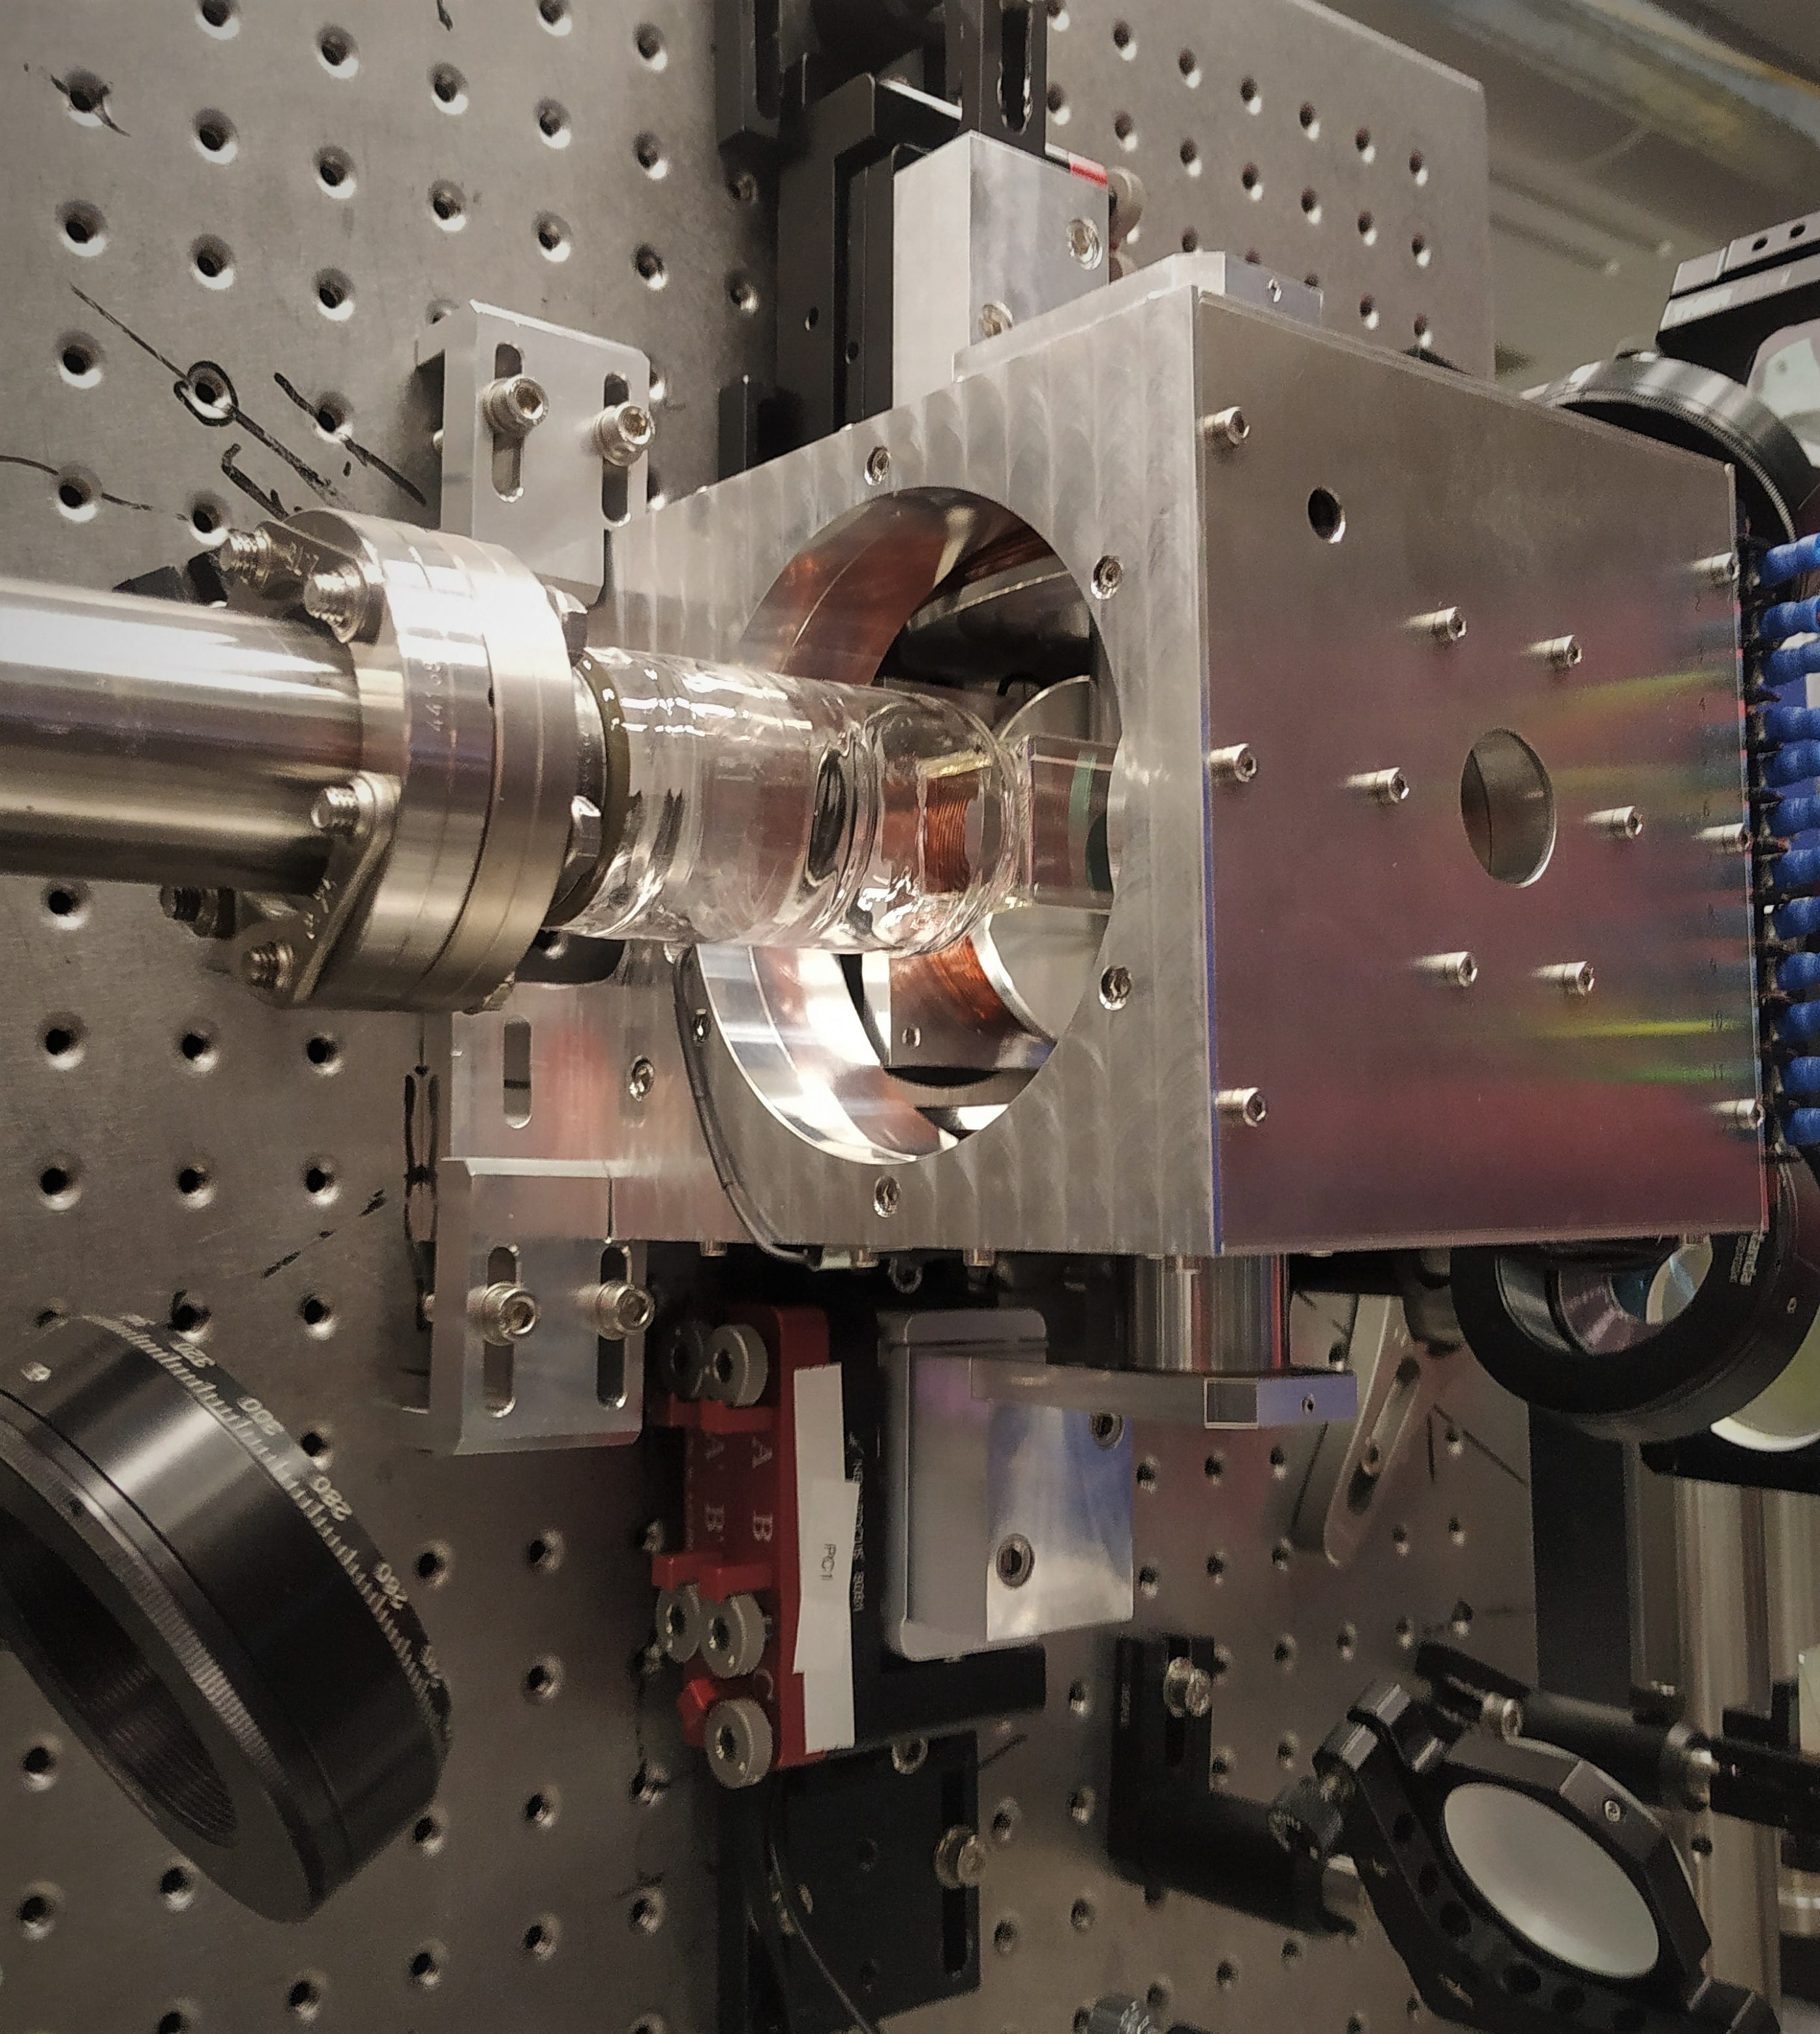
\includegraphics[height=6cm]{figures/Coils.jpg}
		\caption{}
		\label{fig:CoilsSetup}
	\end{subfigure}
	\caption{\textbf{a)} CAD drawing of the vacuum vessel connected to the glass cell on the right. 
	Around the glass cell, 4 out of 6 MOT beams are shown along with the magnetic field coils and a single microscope objective on the bottom. 
	CAD drawing by Eddy Rietman.
	\textbf{b)} Housing for the magnetic field coils, as well as a microscope on a 5-axis stage on bottom and top.}
\end{figure}



\section{Laser System}\label{sec:LaserSystem}

The atomic species that we selected to cool is \textsuperscript{85}Rb because it is the most abundant.
A \textsuperscript{85}Rb requires a cooling laser detuned from the D-2 line of Rb, as well as a repump laser to cycle back atoms in the cooling transition that end up in the wrong ground state.
The laser system was already in the lab, built primarily by \cite{Reijnders2010}.
It used a separate repump laser (Toptica DL100, $P \sim 100$mW) from the trapping/cooling laser (Toptica DLX100, $P \sim 500$mW). 

After numerous components from the repump laser system broke, we decided to omit the seperate repump laser and put sidebands on the trapping laser using an electro optic modulator (EOM) instead, as the small amount of power lost in the trapping laser is not of critical importance for us.
The laser system is sketched in \cref{fig:RbLaserSetup}. 
The fiber on the lower left is where previously both the trapping and repump laser would be fiber coupled for a frequency offset lock system, which we replaced by a (fiber coupled) wavemeter. 

The system consists of a laser detuned by an acousto-optic modulator. For long term stability, the laser is frequency locked using a modulation transfer spectroscopy setup \cite{McCarron2008,Reijnders2010}.
In order for the laser to be in resonance with the Rb spectroscpopy cell, an AOM is used with the same frequency as the AOM going to the MOT. 


In order to make the sidebands, an EOM was used. 
An EOM uses phase modulation to create sidebands with shifted frequencies. 
The amount of sidebands is determines by the modulation depth.
The power in the various sidebands as a function of the modulation index $\epsilon$ is described by \cite{McCarron2008}

\begin{equation}
    E = E_0 \left[
        \sum_{n=0}^{\infty} J_n(\eta)\sin{(\omega_c+n\omega_n)t}+
        \sum_{n=1}^{\infty} (-1)^n J_n(\eta) \sin{(\omega_c-n\omega_m)t}
    \right]
\end{equation}

where $t$ is time and $\omega_c$ the carrier frequency. If $\epsilon <1$ most of the power is contained in the zeroth order (unmodulated) beam and a small fraction is contained in the first sidebands.
The sidebands are always symmetric from the zeroth order, but we only use one of them, the other is wasted. 

The EOM\footnote{7Qubig EO-Rb85-3K} was fed a $f = 2915$ MHz signal provided by a harmonic synthesizer RF \footnote{DS instruments SG6000PRO} providing a signal of $-6.9$dbm.
This signal was amplified by a 45 dB amplifier \footnote{Minicircuits ZHL-16W-43+} which should provide some $\sim 10$\% of power in the first sidebands \cite{Rens2014}, which should be a sufficient amount of power for a repump laser. 

\begin{figure}
    \centering
    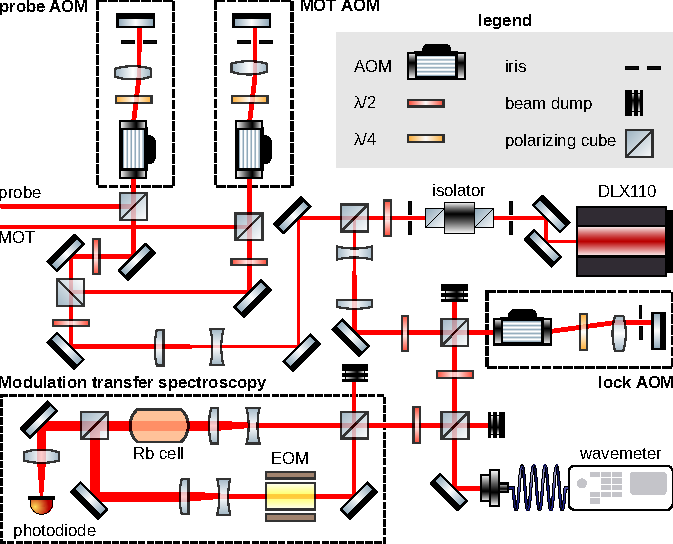
\includegraphics[width=\linewidth]{figures/RbLaserSetup.pdf}
    \caption{Laser system for the trapping and repump laser system for \textsuperscript{85}Rb. The bulk was already built by \cite{Reijnders2010}. All beam splitter cubes shown are polarizing. The Rb vapor cell is heated to 150${^{\circ}}$C.}
    \label{fig:RbLaserSetup}
\end{figure}


\section{Characterizing the MOT}\label{sec:MOTresult}
   
We estimate the number of captured atoms in the MOT by counting the number of counts on our \ac{CCD}, subtracting background counts by turning off the field. 
We obtain the counts by integrating over all pixels $\sum_j p_j$, correcting for exposure time $\tau_s$, camera gain $G$ and sensitivity.
The camera sensitivity constant $C$ was determined to be $6 \cdot 10^3$ counts per photon and was calibrated using a variety of ND filters and a laser at 780 nm of known intensity. The total number of atoms is now
 
 \begin{equation}
     N = \frac{2}{2\pi\gamma} \frac{1}{\beta} \frac{4\pi l^2}{R^2} \sum_j \frac{p_j}{\tau_s G C}
 \end{equation}
 
 where $\gamma$ is the linewidth of the D1 transition of Rb-85, $\beta ~0.6$ is a parameter taking into account photon loss of the glass cell and bandpass filter, $l$ is the distance from the MOT to the collection lens and $R$ is its radius. 
 
The collection angle $\eta$ is $2\pi(1-cos{\alpha})/4\pi$ where $\alpha$ is the maximum angle from the optical axis of the imaging system. $\alpha=\arcsin{0.5}$ the collection angle is $\eta = 0.067$

\section{Tweezer Arrays}\label{sec:Tweezers}

\begin{figure}
    \centering
    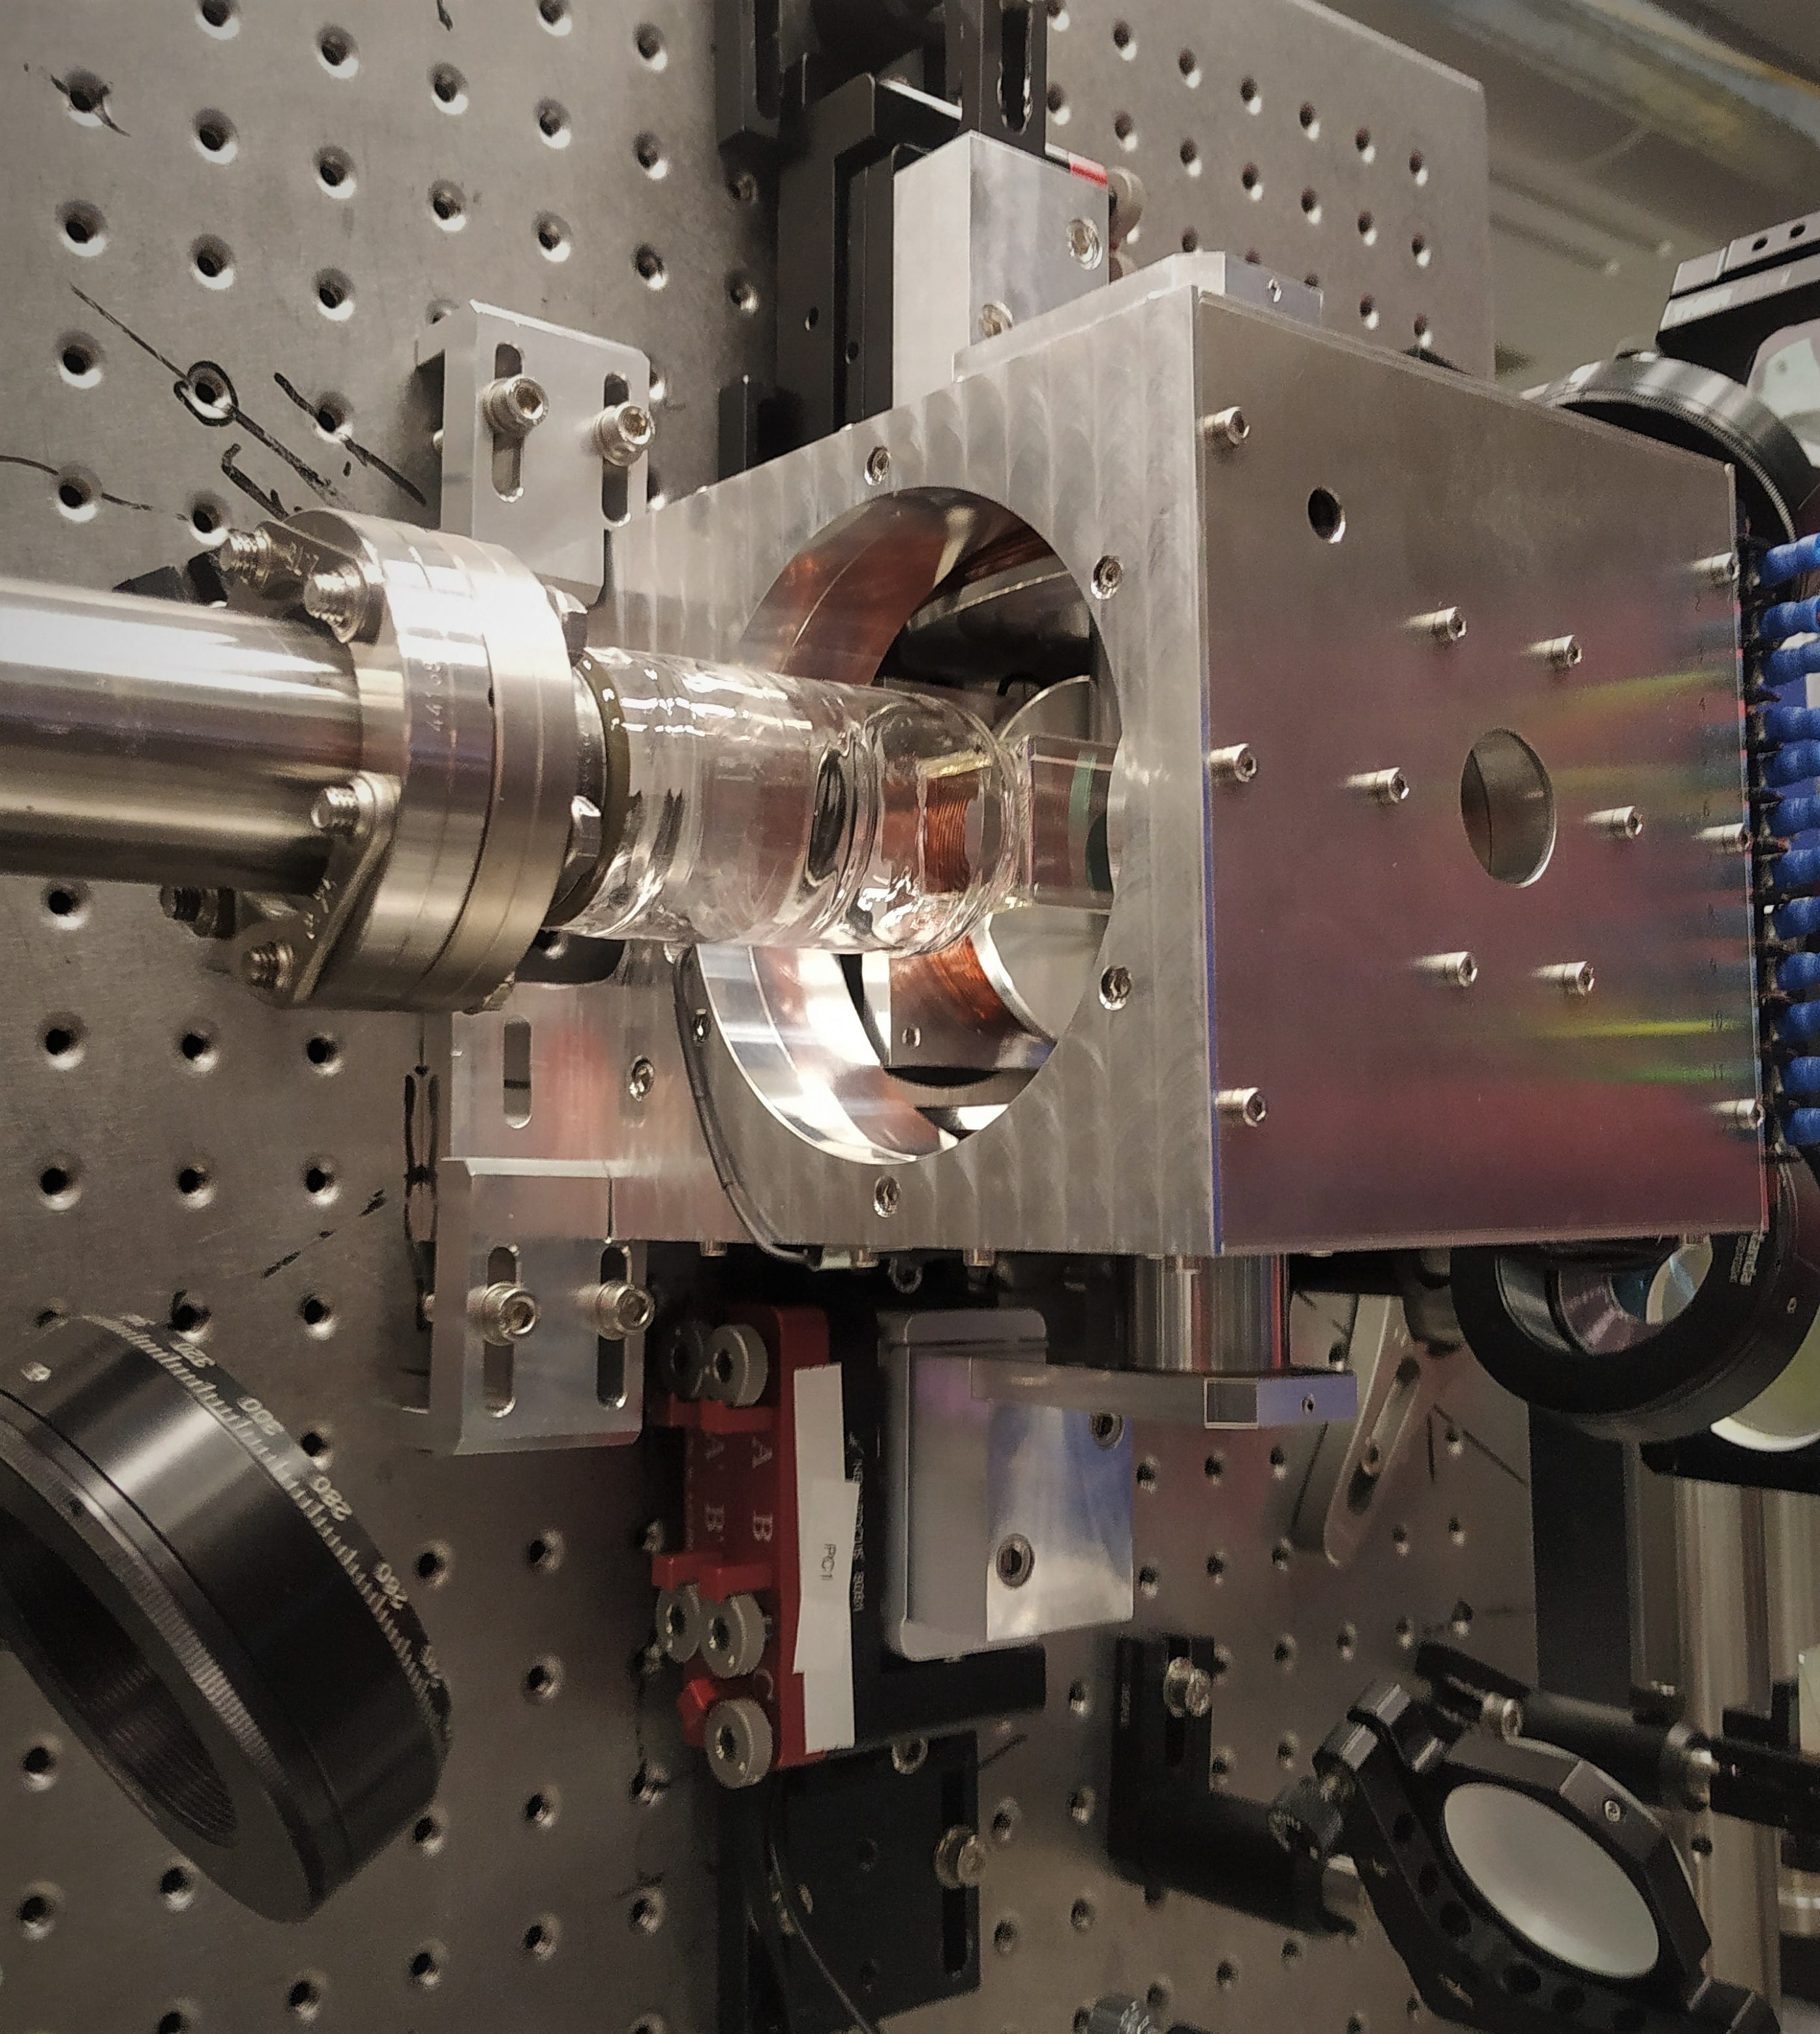
\includegraphics{figures/Coils.jpg}
    \caption{Caption}
    \label{fig:my_label}
\end{figure}

\subsection{Overlapping the MOT with the tweezer}

\begin{itemize}
    \item Top camera: get focus more or less right with 50 mm lens, as well as align tweezer
    \item Scan tweezer over resonance, try to see off balance of MOT from side camera. 
\end{itemize}

\section{Imaging Tweezer Arrays}\label{sec:TweezerImaging}



